\chapter{Data jízdních řádů}\label{kapitola-1}

V~této kapitole řešíme naši potřebu přístupu k~datům, zmíněnou jíž v~sekci~\ref{problemyKReseni-data}.

Tato data jsou dostupná v~různých datových formátech, v~České republice například ve formátu JDF (Jednotný datový formát). Tento a~jemu podobné proprietární formáty však sdílí stejnou nevýhodu. Aplikace pracující s~nimi buď nejsou schopny pracovat s~daty od jiných zprostředkovatelů, nebo musí vytvářet netriviální adaptéry. Takový přístup je zcela nepřípustný, zvláště existují-li alternativy.

Vhodnou alternativou je formát GTFS \citep{gtfs}. Tento formát je spravovaný společností Google a~je ve světě v~podstatě standardem pro popis jízdních řádů.

\section{Zdroje dat}

Za účely vývoje aplikace je vhodné pracovat s~daty, která nám jsou co možná nejbližší, proto budeme pracovat s~daty jízdních řádů v~České republice. Taková data, ve vhodném formátu GTFS \citep{gtfs}, poskytuje společnost Pražské integrované dopravy \citet{pidData}.

Dalším zdrojem dat, nejen pro Českou republiku, je \url{https://transitfeeds.com/}. Vůbec největším zdrojem jednotných dat, se kterými budeme pracovat jsou GTFS for Germany, dostupné na \url{https://gtfs.de/en/feeds/de\_nv/}.

\section{GTFS}\label{gtfs-popis}

Formát GTFS je rozšířením formátu CSV (Comma-separated values). GTFS nevynucuje typ dat, nedá se tedy spoléhat na to, že např. \textbf{id} budou uložena jako čísla. Všechna data z~formátu GTFS, relevantní pro náš problém, jsou zobrazena na obrázku~\ref{fig:gtfs-data}.

\begin{figure}[ht]
    \centering
    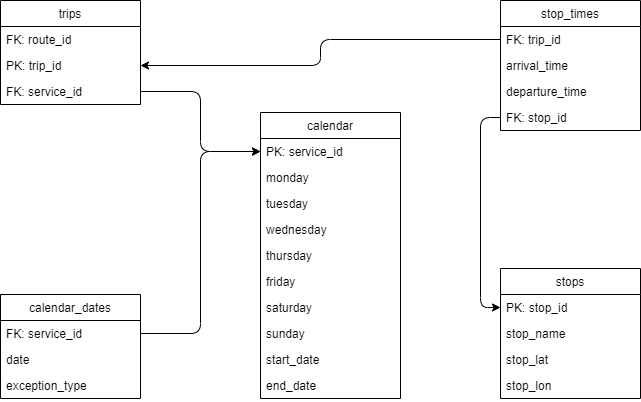
\includegraphics[width=0.75\textwidth]{../img/gtfs-data}
    \caption{Relevantní obsah souborů ve formátu GTFS.}
    \label{fig:gtfs-data}
\end{figure}

Následuje krátký popis nejdůležitějších rysů každé z~používaných složek.
\begin{itemize}
    \item Soubor stops.txt obsahuje geografické souřadnice ve formátu WGS84 (World Geodetic System), ty použijeme k~vizualizaci a~ke generování přestupů. Formát GTFS sice obsahuje přestupy v~transfers.txt, ty však obsahují jen oficiální přestupy, ne všechny možné.
    
    Mezi zastávkami mohou existovat takové zastávky, na kterých nestaví žádný spoj. Takové zastávky budeme chtít odstranit.
    
    \item Soubor stop\_times.txt obsahuje informace o~příjezdu a~odjezdu z~jednotlivých zastávek. Dle specifikace formátu GTFS, může časový formát příjezdů a~odjezdů přesahovat klasický 24 hodinový formát. Taková situace nastává u~spojů, které jedou souvisle přes půlnoc.

    \item \textbf{Route\_id} ze souboru trips.txt identifikuje GTFS trasu, pod kterou patří skupina jízd. 
    
    \textbf{Route\_id} společně se všemi zastávkami, přes které trasa jede, použijeme k~identifikaci pozměněného významu trasy, který používáme v~následujících kapitolách.
    
    \item Soubor calendar.txt přiřazuje k~jízdě dny, kdy je provozována. Každý řádek v~kalendáři má navíc omezenou platnost. Podle GTFS best practices, popsaných na adrese \url{https://gtfs.org/schedule/best-practices/}, by měla být minimální platnost nejméně 7 dnů.

    \item V~souboru calendar\_dates.txt jsou explicitně vypsány výjimky, kdy je jízda provozována a~podle kalendáře by být neměla, nebo naopak kdy jízda není provozována a~podle kalendáře by být měla.
\end{itemize}